\subsection{Internal Generation Procedure Control}
\label{app:internal-generation}
This supplementary comparison varies the generation procedure within the
Agora implementation. Both conditions use its world representation and
rendering conventions; they are not independent world-generation systems.
The total generation budgets also differ, so this is a procedure control,
not a compute-matched component ablation. The returned results below are
retained in full and must not be interpreted as Agora's performance against
an external system.
For each item, a preference for Agora scores 1, a tie 0.5, and a baseline
preference 0; ``Not sure'' is excluded from that item's preference denominator
and reported separately. We average within each request and then equally
across all ten requests, as specified in the released workbook. This prevents
the request receiving four ratings from dominating the overall estimate.

\begin{table}[t]
\centering\small
\setlength{\tabcolsep}{3.2pt}
\begin{tabularx}{\columnwidth}{@{}Yrrrrr@{}}
\toprule
Item & Full & Base & Tie & ? & Score \\
\midrule
Explore & 7 & 13 & 0 & 0 & 40.0\% \\
Clarity & 8 & 11 & 1 & 0 & 32.5\% \\
Scene fit & 7 & 12 & 0 & 1 & 37.5\% \\
\bottomrule
\end{tabularx}

\caption{Structure judgments from ten eligible returns. Full and Base denote Agora
and the single-pass baseline, irrespective of randomized A/B labels; ? = Not
sure. Counts pool twenty comparisons per item. Score is Agora's
\emph{equal-request} mean, not a pooled vote fraction.
No population superiority is inferred from these small counts.}
\label{tab:human-structure}
\end{table}

Respondents select the baseline in thirteen of twenty exploration choices,
versus seven for Agora. Agora's equal-request preference is 40.0\% for
exploration, 32.5\% for world clarity, and 37.5\% for place--scene fit
(Table~\ref{tab:human-structure}). These observations favor the single-pass condition on the displayed
containment diagrams. They neither benchmark Agora against a separate system
nor measure the contribution of its shared representation, renderer, or
runtime. A causal claim about decomposition would additionally require
equalized budgets and controlled retries.

The pattern varies by request (Figure~\ref{fig:human-structure}). Both Tidal
raters prefer Agora for exploration. All four Clockwork raters prefer the
baseline for exploration while choosing Agora for clarity. Understandability
and desire to explore are thus distinguishable judgments in these returns;
we do not sum them into a single quality score. One or two raters on most
requests cannot identify why a design was preferred, and the diagram omits
institutions, social behavior, and actual play. Equal-compute generation and
interactive evaluation remain separate open tests.

\begin{figure*}[t]
\centering
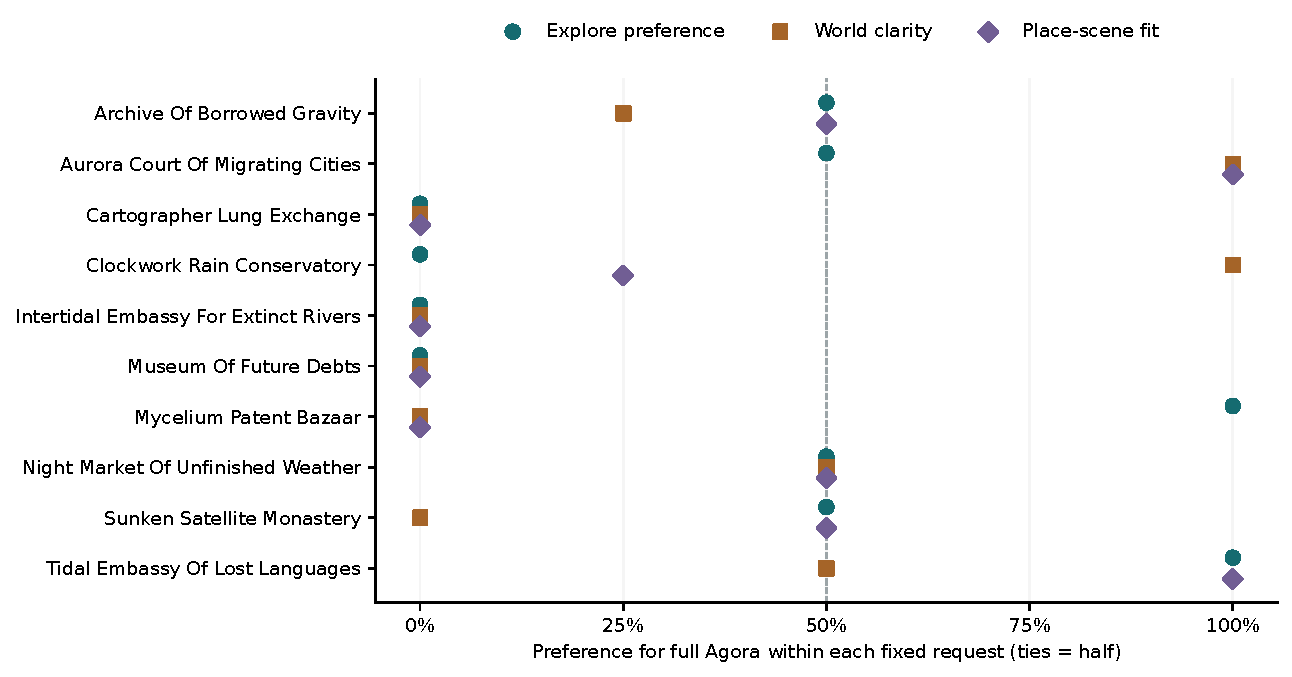
\includegraphics[width=\textwidth]{figures/human_structure_preferences.pdf}
\caption{\paneltitle{World structure: preferences vary by request and item.}
Each point is the fraction favoring full Agora for one request and question,
with a half vote for a tie. The analysis includes 20 comparisons: seven
requests have two raters, two have one, and Clockwork has four. For Tidal
scene fit, one of two raters selects Not sure. These are descriptive fixed-
artifact scores; the dashed line marks equal preference, not a significance
threshold.}
\label{fig:human-structure}
\end{figure*}
